\subsection*{Modelle in der Wissenschaft}
Ein Ansatz zur mathematischen Betrachtung der Krankheitsausbreitung ist das SIR-Modell von William O. Kernack und Anderson Gray McKendrick.\\
Es ist 1927 als Teilgebiet der Epidemiologie entstanden, die sich mit der Verbreitung sowie den Ursachen und Folgen von gesundheitsbezogenen Zuständen und Ereignissen in Bevölkerungen oder Populationen beschäftigt.\\
Da sich das Programm mit derselben Problemstellung befasst, ist ein Vergleich naheliegend.
Dieser soll anhand eines konkreten Beispiels angewandt werden, bei dem beide Modelle mit denselben Daten eine Prognose über die Entwicklung einer Krankheit liefern sollen.\\
Der Vergleich soll eine Einschätzung der Repräsentativität, des dem Projekt zugrunde liegenden Programms ermöglichen und Schwächen und Stärken der beiden Herangehensweisen herausstellen.\\
Bevor das Szenario mit beiden Herangehensweisen vorgestellt wird, wird in diesem Abschnitt das SIR-Modell erläutert. Anschließend wird darauf aufbauend erklärt warum wir uns gerade für den Vergleich des dem Projekt zugrunde liegendem Programm mit diesem Modell entschieden haben.

\subparagraph{Das SIR-Modells}
\begin{figure}
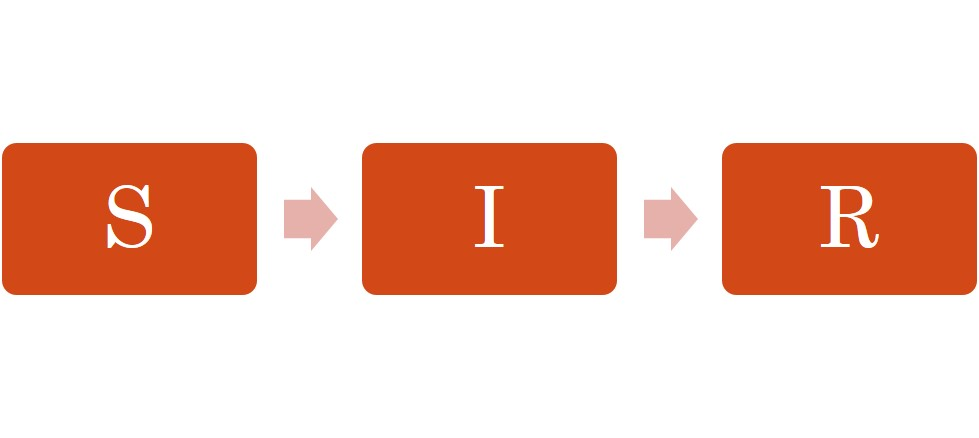
\includegraphics[width= 0.3\textwidth]{./images/SIR-Modell.jpg}\caption{Zustandsmodell des SIR-Modells}
\end{figure}
Das SIR-Modell ist eine mathematische Herangehensweise, bei der der Krankheitsverlauf statisch über feste Funktionen errechnet wird.
Beim SIR-Modell wird eine geschlossene Gruppe N an Individuen betrachtet. Die Anzahl der Personen in N ist die Gesamtgröße der Bevölkerung.
Diese setzt sich aus gesunden, kranken und 'R'-Individuen zusammen, sodass gilt:
\begin{equation}
N = S + I + R
\end{equation}
. Das heißt: Die Bevölkerung wird in drei Zuständen klassifiziert:
\begin{itemize}
\item \textbf{S (Susceptible)} Anfällige Individuen, die innerhalb der Bevölkerung Infiziert werden können.
\item \textbf{I (Infected)} Infizierte Individuen, die Anfällige anstecken  oder in den R-Zustand übergehen können.
\item \textbf{R (Recovered)} Der letzte Zustand ist der R-Zustand. Ein infiziertes Individuum, was in den R-Zustand übergeht, bleibt im R-Zustand. Es gibt keinen Übergang aus dem R-Zustand zurück in einen der anderen Zustände. Der R-Zustand kann von daher Individuen beschreiben, die aus Epidemiologischer Sicht keinen Einfluss mehr auf den Rest der Gesellschaft haben. Dies könnten z.B. immunisierte, tote oder isolierte Individuen sein.
\end{itemize}
Zur Visualisierung des Krankheitsverlauf in einer Bevölkerung kann geeigneter Weise ein Koordinatensystem benutzt werden, dass die Anzahl der Individuen in Relation zur Zeit setzt.
Für jede Zustandsgruppe wird ein Graph in das Koordinatensystem gezeichnet, sodass ablesbar wie viele Individuen zu einem Zeitpunkt krank, gesund oder im "R"-Zustand sind.\\
Die Verteilung der Individuen in die jeweiligen Zustandsklassen ändert sich mit dem Fortschritt der Zeit, ist die Krankheit nicht ausgestorben, die Infektionsrate oder "R"-Übergangsrate größer null und nicht alle Individuen im 'R'-Zustand.
Für jeden Zeitschritt t wird die Anzahl der Individuen in den Zustandsklassen neu berechnet.\\
Beispielsweise erkranken nach einem Zeitschritt drei neue Individuen und ein Individuum stirbt. Damit nimmt die Gruppe S um drei Individuen ab, die Gruppe I wächst entsprechend um drei Individuen und gibt gleichzeitig ein Individuum an die Gruppe R ab, sodass sich die Verteilung von beispielsweise S = 5, R = 5 und I = 5 nach einem Zeitschritt zu S = 2, I = 7 und R = 6 ändert.

\subparagraph{Berechnung der Entwicklung}
Damit die Verteilung sinnvoll berechnet werden kann, werden Kennzahlen über die Krankheit benötigt, die das Krankheitsprofil widerspiegeln. Dabei wird für das SIR-Modell die Infektionsstärke und die "R"-Übergangsrate benötigt.
Über die Infektionsstärke wird dann die Ansteckungs-Kontakt-Rate ermittelt. Diese ist die Wahrscheinlichtkeit mit der ein Individuum mit X Kontakten pro Zeitschritt in einer Bevölkerung erkranken kann.
\begin{equation}
b = ( \lambda * KaT) / N
\end{equation}
Dabei ist die Anzahl der Kontakte je nach Krankheitsübertragungsweg zu unterscheiden. Bei Krankheiten die über Tröpfcheninfektion übertragen werden reicht Hände schütteln, die Übergabe von Geld oder sogar das Zusammensein in einem Raum zur Infektion. In diesem Szenario wird oft ein Durchschnittswert von 8 Menschen am Tag genommen. Bei Krankheiten mit anderen Übertragungswegen z.B. AIDS muss der Austausch von Körperflüssigkeiten zur Infektion stattfinden. Diese ist im Durchschnitt natürlich deutlich geringer als bei Tröpfcheninfektion und verändert die Ansteckungs-Kontakt-Rate immens.
Über die Ansteckungs-Kontakt-Rate kann die Basisreproduktionsrate ermittelt. Diese beschreibt die Wahrscheinlichkeit für ein Individuum sich zu infizieren, bei wachsender Anzahl der Infizierten.
\begin{equation}
R0 = ( b * N ) / \gamma
\end{equation}

Hat man die beiden Größen ermittelt, können die Funktionen für die drei Zustände S, I und R über einen Zeitraum ermittelt werden. 
Es gilt:

\begin{equation}
\end{equation}

%\subparagraph{Szenario} -hidden
%/*
%Das Szenario spielt in einem kleinen Dorf mit 10150 Einwohnern zur Zeit des Mittelalters. Damals hat die Pest, oft bezeichnet als "Schwarzer Tod" von 1347 bis 1353 ein Drittel des europäischen Bevölkerung das Leben gekostet hat. 
%Während einige Landstriche komplett entvölkert wurden und in Italien fast jeder 5. der Krankheit erlag starb in Deutschland jeder 10.an der Infektionskrankheit. 
%Aufgrund der regionalen Unterschiede und der wenigen verlässlichen Daten ist es besonders schwer die die Kennzahlen der Krankheit möglichst Realitätsnah wiederzugeben, insbesondere wenn die Krankheit tödlich ist.
%Die Diagnose Pest war damals gleichzusetzen mit dem Todesurteil, da nur ein sehr geringer Teil der Bevölkerung diese Krankheit mit den medizinischen Stand überleben konnte.
%Für den Vergleich wird angenommen, dass die Krankheit eine Infektionsrate von 33\% hat. Zudem stirbt ein erkranktes Individuum pro Runde zu 70\% an seiner Krankheit. Die Wahrscheinlichkeit zu genesen oder sogar Resistent zu werden liegt jeweils bei 2\%. */ 

\subparagraph{Warum gerade das SIR-Modell?}
Bei dem Vergleich mit bekannten Modellen aus der Wissenschaft drängt sich zunächst die Frage auf warum im Rahmen des Projektes gerade der Vergleich mit dem SIR-Modell angestellt wurde und nicht mit einem anderen Modell zur Darstellung eines Krankheitsverlauf.\\
Wie genau ein mathematisches Modell die Krankheitsausbreitung in einer Gesellschaft beschreibt, hängt sehr davon ab, wie viel Realismus und damit wie viele Annahmen hineingesteckt werden.\\
Da in der Medizin viele Einflüsse zunächst vernachlässigt werden müssen, nicht bekannt sind oder die Krankheit sich mit der Zeit durch mutierende Viren verändert, haben die Modelle sehr selten einen endgültigen Charakter. Darüber hinaus sind Krankheiten in ihrer Entwicklung so unterschiedlich, dass es sehr oft möglich und manchmal nötig ist, die Modelle weiter zu verfeinern und anzupassen, wobei unterschiedliche Krankheiten unterschiedliche Modelle erfordern können. 
So kann es möglich sein, dass eine Verfeinerung eines Modells, dass für 2 Krankheiten annehmbare Näherungswerte liefert, für eine Krankheit sehr gute Näherungen bringt, aber dafür bei der anderen Krankheit versagt.\\
Mit anderen Worten: Eine Krankheit kann mit all ihren Eigenschaften sehr realitätsnah abgebildet werden, aber möglicherweise bei einer anderen Krankheit schon wieder versagen. Von daher ist nicht das Modell, sondern das zugrunde liegende Szenario entscheidend für die Wahl des Vergleichsmodells. Eine sinnvolle Vorgehensweise ist es daher erst ein Szenario zu erschaffen und dieses dann mit einem geeigneten Modell abzubilden.\\ 
Im Rahmen unserer Projektes wurde sich für die Mittelalterpest entschieden.\\ 
Die Mittelalterpest war im 14. Jahrhundert gleichzusetzen mit einem Todesurteil. Beinahe jedes Individuum erlag nach einiger Zeit seiner Krankheit. Aus diesem Grund passt die Natur des Modells sehr gut zum vorgegebenen Szenario und dem Krankheitsprofil der Pest: Ein gesundes Individuum kann infiziert werden und dann sterben. In diesem Fall bildet der "R"-Zustand, die Anzahl der verstorbenen Individuen ab.\\
Mit einem anderen Szenario wäre es sinnvoll gewesen ein anderes Modell zu betrachten. 
Andere Modelle, die in der mathematischen Biologie angewendet werden sind z.B. das SI-Modell oder SIS-Modell.\\
Das Zustandsmodell im SIS-Modell ist im Gegensatz zum SIR-Modell zyklisch. Es gibt nur zwei Zustände: Anfällig und Infiziert. Anfällige Individuen können infiziert werden und dann wieder genesen. Sind sie genesen können sie wiederum infiziert werden. Damit ist das SIS-Modell vor allem geeignet für bakterielle Erkrankungen wie z.B. Tuberkulose, bei der Individuen wieder genesen, aber keine Immunität entwickeln. \\
\begin{figure}
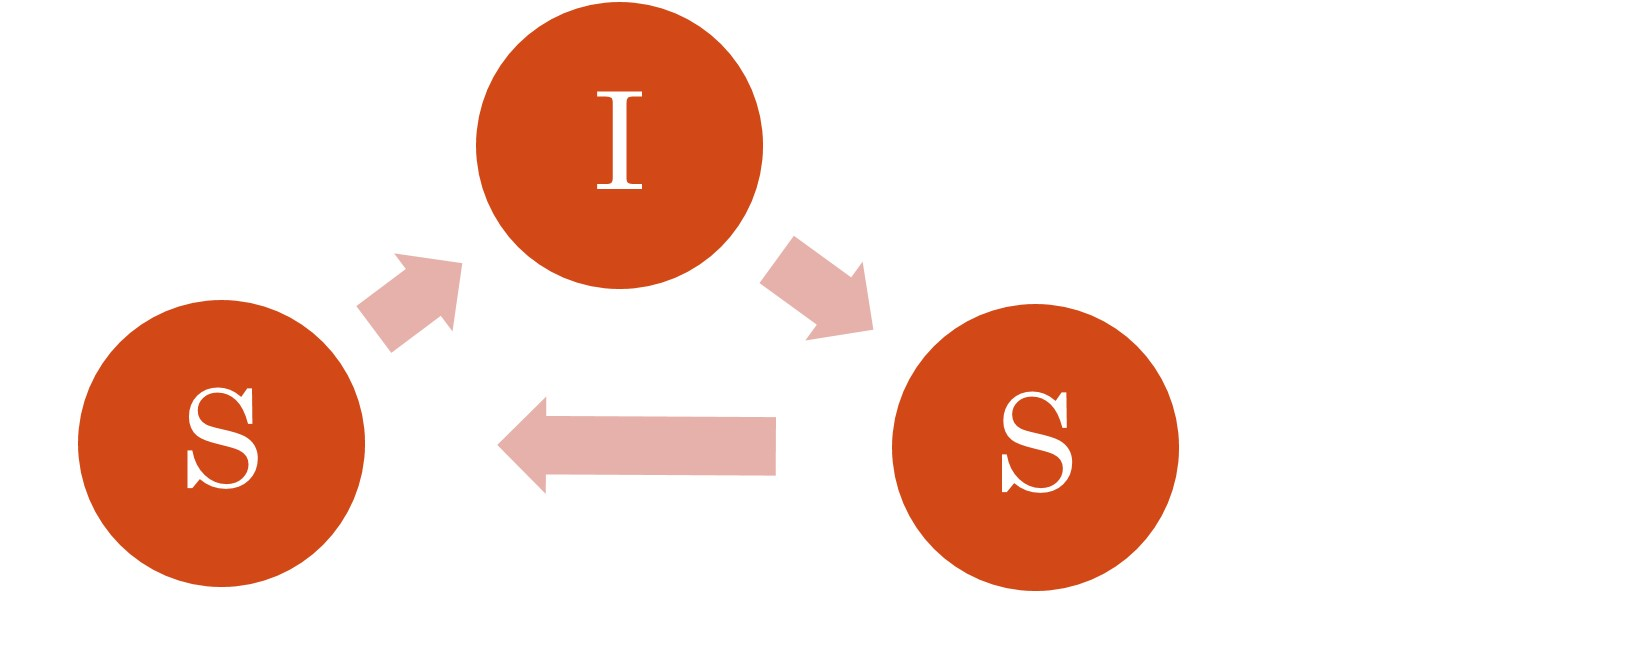
\includegraphics[width= 0.3\textwidth]{./images/SIS-Modell.jpg}\caption{Zuständsmodell des SIS-Modells}
\end{figure}
Das SI-Modell hat ebenfalls die beiden Zustände Anfällig und Infiziert, aber ist nicht zyklisch. Es können lediglich Individuen Infiziert werden. Diese bleiben endgültig im Zustand I.\\ 
Das SI-Modell ist also sinnvoll, wenn Individuen lediglich an einer Krankheit erkranken und nicht wieder genesen, aber auch nicht sterben. Das entsprechende Szenario, wäre beispielsweise ein Zombie-Virus, wie der im Programm implementierte "I am Legend - Virus".\\
Damit wird der erste Vorteil der Herangehensweise im Programm sichtbar: Während bei der mathematischen berechnen für jedes Modell ein anderes Modell gewählt werden muss, um möglichst nah an der Realität zu bleiben, ist das Programm auf mehrere Szenarien mit Heilung, Toten, Resistenten etc. anwendbar.